\documentclass[a4paper,11pt]{article}
\usepackage{amsmath,amsthm,amsfonts,amssymb,amscd,amstext,vmargin,graphics,graphicx,tabularx,multicol} \usepackage[french]{babel}
\usepackage[utf8]{inputenc}  
\usepackage[T1]{fontenc} 
\usepackage[T1]{fontenc}
\usepackage{amsmath,amssymb}
\usepackage{pstricks-add,tikz,tkz-tab,variations}
\usepackage[autolanguage,np]{numprint} 
\usepackage{color}
\usepackage{ulem}

\setmarginsrb{1.5cm}{0.5cm}{1cm}{0.5cm}{0cm}{0cm}{0cm}{0cm} %Gauche, haut, droite, haut
\newcounter{numexo}
\newcommand{\exo}[1]{\stepcounter{numexo}\noindent{\bf Exercice~\thenumexo} : \marginpar{\hfill /#1}}
\reversemarginpar


\newcounter{enumtabi}
\newcounter{enumtaba}
\newcommand{\q}{\stepcounter{enumtabi} \theenumtabi.  }
\newcommand{\qa}{\stepcounter{enumtaba} (\alph{enumtaba}) }
\newcommand{\initq}{\setcounter{enumtabi}{0}}
\newcommand{\initqa}{\setcounter{enumtaba}{0}}

\newcommand{\be}{\begin{enumerate}}
\newcommand{\ee}{\end{enumerate}}
\newcommand{\bi}{\begin{itemize}}
\newcommand{\ei}{\end{itemize}}
\newcommand{\bp}{\begin{pspicture*}}
\newcommand{\ep}{\end{pspicture*}}
\newcommand{\bt}{\begin{tabular}}
\newcommand{\et}{\end{tabular}}
\renewcommand{\tabularxcolumn}[1]{>{\centering}m{#1}} %(colonne m{} centrée, au lieu de p par défault) 
\newcommand{\tnl}{\tabularnewline}

\newcommand{\trait}{\noindent \rule{\linewidth}{0.2mm}}
\newcommand{\hs}[1]{\hspace{#1}}
\newcommand{\vs}[1]{\vspace{#1}}

\newcommand{\N}{\mathbb{N}}
\newcommand{\Z}{\mathbb{Z}}
\newcommand{\R}{\mathbb{R}}
\newcommand{\C}{\mathbb{C}}
\newcommand{\Dcal}{\mathcal{D}}
\newcommand{\Ccal}{\mathcal{C}}
\newcommand{\mc}{\mathcal}

\newcommand{\vect}[1]{\overrightarrow{#1}}
\newcommand{\ds}{\displaystyle}
\newcommand{\eq}{\quad \Leftrightarrow \quad}
\newcommand{\vecti}{\vec{\imath}}
\newcommand{\vectj}{\vec{\jmath}}
\newcommand{\Oij}{(O;\vec{\imath}, \vec{\jmath})}
\newcommand{\OIJ}{(O;I,J)}

\newcommand{\bmul}[1]{\begin{multicols}{#1}}
\newcommand{\emul}{\end{multicols}}


\newcommand{\reponse}[1][1]{%
\multido{}{#1}{\makebox[\linewidth]{\rule[0pt]{0pt}{20pt}\dotfill}
}}

\newcommand{\titre}[5] 
% #1: titre #2: haut gauche #3: bas gauche #4: haut droite #5: bas droite
{
\noindent #2 \hfill #4 \\
#3 \hfill #5

\vspace{-1.6cm}

\begin{center}\rule{6cm}{0.5mm}\end{center}
\vspace{0.2cm}
\begin{center}{\large{\textbf{#1}}}\end{center}
\begin{center}\rule{6cm}{0.5mm}\end{center}
}



\begin{document}
\pagestyle{empty}
\titre{Contrôle 2 : Calcul littéral, notion de fonctions et trigonométrie}{Nom}{Prénom}{Date}{Classe}

\vspace*{0.2cm}

\exo{2.5}

\initq \q Développer et réduire $M = (9 - x)(2x + 6) - 3 (x - 4)$.  \\

\q Calculer l'expression M pour $x=-1$.\\

\vspace*{0.3cm}

\exo{2.5} Factoriser les expressions suivantes : 

\bmul{2}


 $Z = (2x - 3)(6 - x) + (3x - 2)(2x - 3)$\\


\columnbreak

 
$ E = (4 + x)^{2} - (4 + x)(3x + 1)$

\emul

\vspace*{0.2cm}

\exo{2} Pour chacune des questions, entourer en bleu la bonne réponse :
\begin{center}
\includegraphics[scale=1]{QCM.eps} 
\end{center}

\vspace*{0.5cm}

\exo{3}\\

Voici un tableau de valeurs : \hspace*{1cm} \begin{tabular}{|c|c|c|c|c|c|c|c|}
\hline 
$x$ & 4 & -3 & 12 & -1 & 2 & 5 & 8 \\ 
\hline 
$f(x)$ & 12 & -6 & 5 & 8 & 4 & 7 & 17 \\ 
\hline 
\end{tabular} 

\vspace*{0.5cm}

\initq \q Recopier et compléter :
\bmul{4}

\qa  $f(-3) =  . . .$

\columnbreak

\qa $f(5) =  . . .$

\columnbreak

\qa $f(. . . ) =  4$

\columnbreak

\qa $f(. . . ) =  5$

\emul

\q Quelle est l'image de 8 par la fonction f ?\\

\q Quel est l'antécédent de 12 par la fonction f ?\\

\vspace*{0.5cm}

\exo{4}

\initq \q Soit h la fonction définie par $h(x) = \dfrac{-x+8}{x^{2}+1}$.\\
Calculer l'image de -2 par la fonction $h$.\\

\q Soit $g : x \mapsto -3x^{2} + 1$.\\

\initqa \qa Calculer $g(1)$.\\

\qa Vérifier par le calcul que l'antécédent de -11 par la fonction $g$ est 2.\\

\qa Est-ce que $h(1) = h(-1)$ ? \textbf{Justifier votre réponse.}\\

\newpage
\vspace*{0.4cm}

\exo{3}

Quand un avion n'est plus très loin de l'aéroport de Toulouse, le radar de la tour de contrôle émet un signal bref en direction de l'avion. Le signal atteint l'avion et revient au radar 0,000 3 seconde après son émission.\\

\initq \q	Sachant que le signal est émis à la vitesse de 300 000 kilomètres par seconde, vérifier qu'à cet instant, l'avion se trouve à 45 kilomètres du radar de la tour de contrôle.\\

\begin{center}
\includegraphics[scale=1]{avion.eps} 
\end{center}


\q La direction radar-avion fait un angle de 5\degre avec l'horizontale. Calculer alors l'altitude de l'avion à cet instant. Arrondir à la centaine de mètres près. (On négligera la hauteur de la tour de contrôle.)\\


\vspace*{0.5cm}



\exo{3}

A, B et C sont trois points d'un cercle tel que [AB] est un diamètre du cercle, AC = 4,5 cm et BC = 3,4 cm.\\


\initq \q Faire une figure en vraie grandeur.\\

\q Le triangle ABC est un triangle rectangle en C. Déterminer la mesure de l'angle $\widehat{CAB}$ dans le triangle ABC. En donner l'arrondi au degré près.\\

\vspace*{0.5cm}

\exo{}(Bonus)

On sait que $tan x =  \dfrac{5}{12}$  et $sin x =  \dfrac{5}{13} $. 
Calculer la valeur exacte de cos x puis vérifier que $(cos x)^{2} + (sin x)^{2} = 1$.






\end{document}
